\section{INTRODUCCIÓN}

\subsection{ANTECEDENTES}
Las tecnologías de la información y la comunicación han sido el inicio de un conjunto de cambios y crecimiento, se encuentran cada vez más extendidas contribuyendo a la reducción de la comunicación sin importar el área geográfica.\\

Jugando un papel muy importante dentro del sector automotriz, las tecnologías de la información y la comunicación han sido necesarias para la evolución de los vehículos en cuestión de seguridad y confort entre otros aspectos, logrando que el vehículo sea capaz de monitorear fallas mediante sensores implementados en él.\\

El primer vehículo era propulsado a vapor y fue creado por Nicholas Joseph Cugnot en 1769 (\cite{UPS-22,UPS-23}). era triciclo con ruedas de madera, llantas de hierro y pesaba 4,5 toneladas, no fue hasta en 1801 aparece el primer taxi a vapor y para 1840 aparecio el primer carro a vapor con capacidad de 18 pasajeros.\\

Después de 20 años el belga Etienne Lenoir en 1860 patentó el primer motor a explosión que fue un punto clave para la evolución, ya que, el motor de combustión interna apareció en 1876 por Karl Benz con forma de triciclo y en 1881 aparece el vehículo eléctrico de Jeantaud utilizando veintiún baterías para su funcionamiento, pasaron dos años y se creó el primer motor de gasolina de alta velocidad construido y diseñado por W.Maybach en 1883.\\ 

En la década de 1890 Henry Ford decidió entrar al negocio de los automóviles. Su primer dolor de cabeza fue la patente obtenida por Baldwin Selden en 1895, que se adueñaba de los derechos de la aplicación del motor de combustión interna a los carros. En EEUU, en 1899 Olds fabricó 400 autos en 6 meses y se convertía en el mayor fabricante de Estados Unidos. Después de cuatro años Spyker construye el primer motor de seis cilindros y el primer vehículo con tracción de cuatro ruedas de los Países Bajos.\\

En 1910 Las firmas Argyll, Crossley, Arrol Johnson e Isotta Fraschini emplean por primera vez frenos a las cuatro ruedas y en 1920 apareció el primer auto SEDAN, no paso mucho tiempo para que en 1924 se construyera el primer vehículo con nombre CHRYSLER, Walter P. Chrysler lanza un auto con su nombre que incluye frenos hidráulicos y motor de alta compresión.\\

En 1981 El completamente nuevo auto ``K'' estaba impulsado por un nuevo motor de 2.2 litros y solo cuatro cilindros. El Chrysler New Yorker del año 1988 fue el primer automóvil americano con ``\textit{Air Bag}'' como equipamiento estándar de seguridad y HONDA empieza el siglo XXI vendiendo el INSIGHT, un híbrido gasolina-electricidad en los Estados Unidos.\\


Hoy en día, el automóvil se ha convertido en un bien de primera necesidad llevando a la industria automotriz a alcanzar niveles extraordinarios de producción en México según la Asociación Mexicana de la Industria Automotriz A.C (\cite{UPS-16}). Tal cual como se muestra en la Figura \ref{Fcero1} la producción es de manera ascendente por cada año que ha pasado.


%
\begin{figure}[H]
%\vspace{0.2cm}
\centering
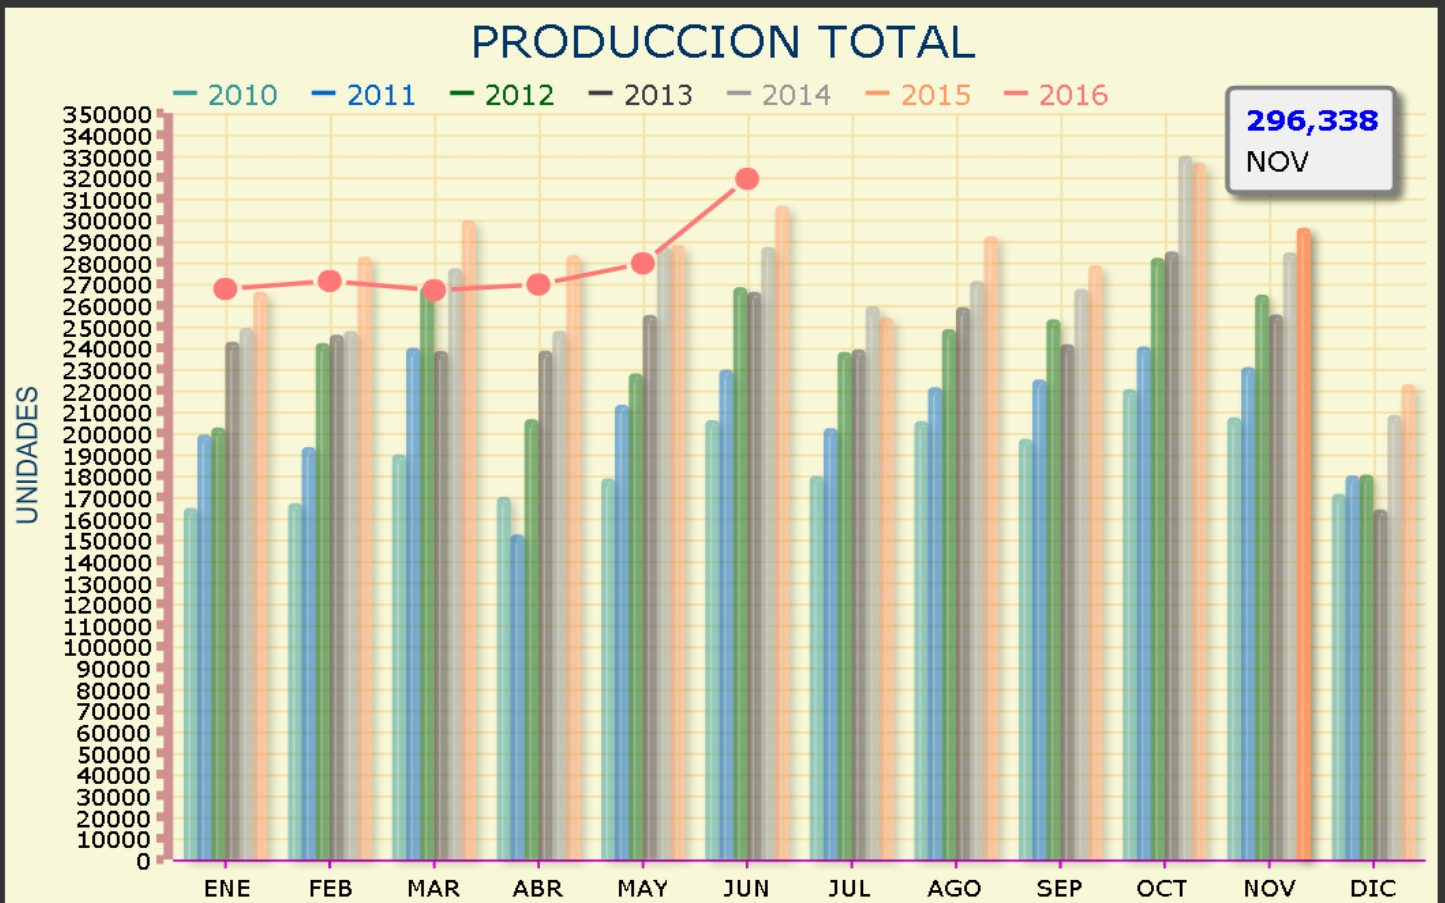
\includegraphics[width=0.7\textwidth]{introduccion/fig14.jpg}
\caption{Gráfica de producción total de vehículos en México \cite{UPS-16}. }
\label{Fcero1}
\end{figure}

En un artículo, la revisar Forbes (\cite{UPS-15}). Anuncio que un estudio de la Consultora IHS arrojó que se espera un crecimiento de 32 \% en la venta de vehículos para el 2021 a nivel mundial comparado con el periodo 2006-2013(557 millones de vehículos), esto hace que la innovación y la optimización de los mismos sea de gran importancia.\\

En la actualidad los automóviles cuentan con una serie de unidades de control que incluyen microprocesadores, tales como la unidad de control del motor, sistema de trasmisión, \textit{airbags}, sistemas de frenos, entre otros.\\


\subsection{DESCRIPCIÓN DEL PROBLEMA}

Actualmente en México se observan muchos vehículos de gama baja que se están deteriorando con el paso del tiempo sin que las personas tengan la intención de repararlos, debido a la gran posibilidad de financiar un carro de mejores características en cuestión de seguridad y confort, aunque implique un gran gasto mediante un plazo largo de cuotas.\\

Esta situación con lleva a una economía más ajustada debido al financiamiento de las agencias vehiculares y los intereses, además de que las personas que desean continuar con su vehículo actual no han encontrado un centro de servicio automotriz que trabaje bajo un método para aumentar las características del vehículo e incorporarle tecnología accesible en respecto a la seguridad y confort del usuario.\\

La compra de un modelo más reciente es la única forma de elevar la experiencia y seguridad del tripulante a la hora de viajar. En México el 46.2 \% de las personas según el Consejo Nacional de Evaluación de la Política de Desarrollo Social tiene pobreza (\cite{UPS-18}). A pesar de la situación económica del país, el registro de vehículos ha estado aumentando año tras año según las estadísticas de el Instituto Nacional de Estadística y Geografía (\cite{UPS-17}). Tal cual se muestra en la Figura \ref{Fcero2}. \\

\begin{figure}[H]
%\vspace{0.2cm}
\centering
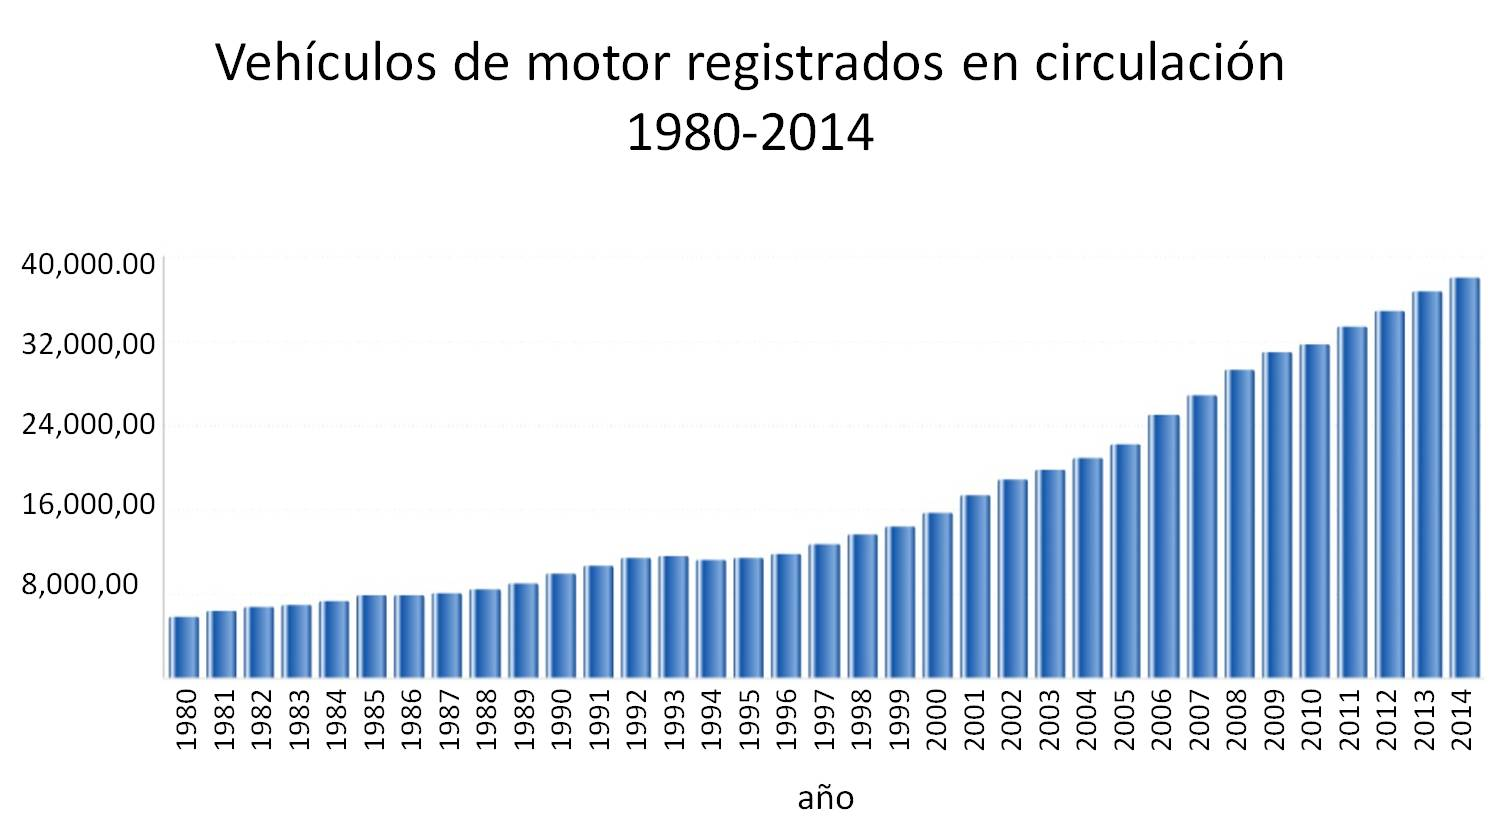
\includegraphics[width=1\textwidth]{introduccion/fig15.jpg}
\caption{Estadísticas de vehículos de motor registrados en circulación \cite{UPS-17}. }
\label{Fcero2}
\end{figure}



La compra de un vehículo modelo más reciente provoca una gran satisfacción durante su uso, sin embargo, el costo se eleva significativamente a su vez que la tecnología se va incluyendo, esto debido al encarecimiento en la compra de algunas piezas o sensores necesarios para el óptimo trabajo del vehículo. \\

También existe un factor muy importante para la economía de los mexicanos que es el alto índice de robos de los vehículos según la Asociación Mexicana de Instituciones de Seguros \cite{UPS-19} fueron 62 mil 533 unidades de autos asegurados robados en el 2015 y para la población es un descontrol económico el adquirir un vehículo sin una planificación de compra.\\



\subsection{JUSTIFICACIÓN}
Las agencias automotrices han procurado desarrollar vehículos con diferente cantidad de tecnología enfocada en el sistema de confort, a pesar de que no es mucha la diferencia de tecnología el precio que encarece el producto es notable.\\

El desarrollar una metodología que permita incluir tecnología actual a vehículos de gama baja y modelos anteriores es una gran oportunidad para que las personas puedan seguir usando su vehículo sin la necesidad de buscar otro por falta de tecnología, seguridad y comodidad.  \\

El restaurar un vehículo actualmente es costo y el valor en el mercado es muy bajo, en cambio si se le agrega tecnología puede llegar a cambiar el nivel de la gama e incluso aumentar el costo en el mercado, aprovechando que la industria automotriz es considerada uno de los pilares de la segunda más grande economía de América Latina y México es uno de los mayores exportadores de vehículos del mundo, según la revista Forbes (\cite{UPS-20}). Además, en otro artículo (\cite{UPS-21}), la revista Forbes menciona que mientras en América Latina las ventas automotrices reportan números rojos, en México crecen 17 \% en el 2015. \\

\subsection{ESTADO DEL ARTE}
Existen trabajos relacionados con incluir tecnología para optimizar, manipular y/o monitorear algún sensor o actuador del vehículo, se consultaron documentos científicos revisando las propuestas, resultados y limitaciones de algunas investigaciones con la finalidad de encontrar trabajos relacionados con los temas de seguridad, confort, monitoreo, automatización y comunicación.\\

Se ha encontrado una gran cantidad de proyectos vehiculares utilizando el sistema global para las comunicaciones móviles (GSM del inglés \textit{Global System for Mobile Communication}) (\cite{UPS-01,UPS-03,UPS-04,UPS-05,UPS-07}). La tecnología GSM permite la manipulación a distancia y es un reto que varios investigadores han aceptado en la actualidad.\\

Ángel Cornejo y Jorge Tintín en el 2010 (\cite{UPS-01}), desarrollaron e implementaron un sistema de telemetría a través de la tecnología GSM en un vehículo Chevrolet OPTRA 2008 monitoreando los parámetros de: i) temperatura, ii) presión de aceite, iii) velocidad de giro del motor y iv) velocidad de desplazamiento. El sistema se construyó mediante tecnología GSM, utilizaron un dispositivo móvil para conectar a la tarjeta electrónica, como medio de comunicación debido al alcance de cobertura de la red móvil. Sin embargo, se tiene un costo por cada acción, para tener en perfecto estado la comunicación Ángel recomienda tener activo un paquete ilimitado de mensajes de texto ya que el agotamiento del servicio de mensajería simple (SMS del inglés \textit{Short Message Service}) provocaría errores en la recepción y envío de datos.\\

En el 2012 Fabián Arancibia y Claudio Urrea (\cite{UPS-02}), implementaron un sistema de teleoperación en un carro de golf eléctrico con la finalidad de sentar las bases para la experimentación e implementación de sistemas de teleoperación. Se realizó un proyecto el cual está constituido por tres bloques básicos los cuales se muestran en la Figura \ref{Funo}. Una combinación un \textit{joystick}, enrutador Wifi, la placa de Arduino Mega y una interfaz electrónica que en conjunto sirve para manejar los actuadores del volante, los pedales, las luces y la bocina.  Utilizando cámaras de red para obtener retroalimentación y visualizar con un margen de retardo de un segundo. Sin embargo, es necesario estar cerca de una red Wifi para poder acceder al sistema de control remoto.\\

%
\begin{figure}[H]
%\vspace{0.2cm}
\centering
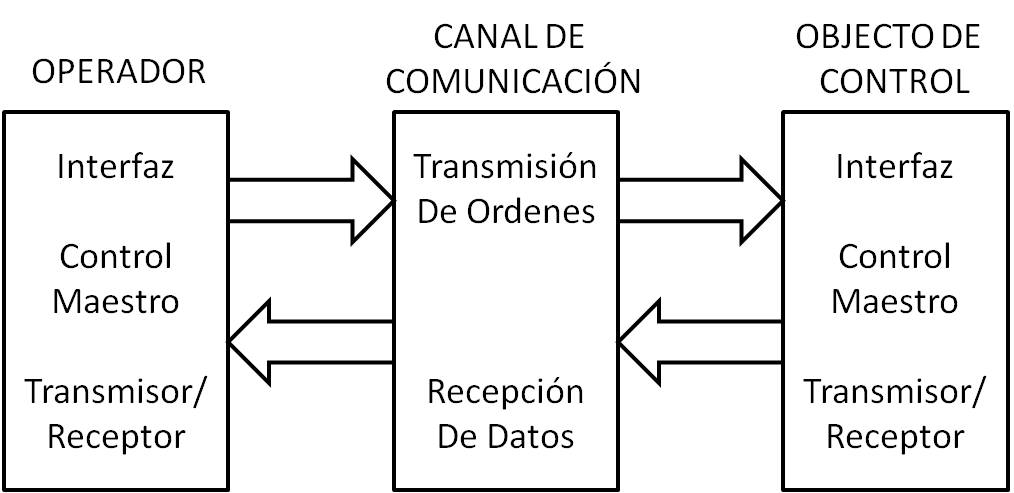
\includegraphics[width=0.6\textwidth]{introduccion/fig1.jpg}
\caption{Diagrama de bloques del sistema. }
\label{Funo}
\end{figure}
%

El tema de seguridad vehicular se ha trabajado sobre la cuestión para bloquear y desbloquear de manera física o mediante un SMS el sistema de encendido del vehículo (\cite{UPS-03,UPS-04,UPS-09}). Utilizando un dispositivo móvil que se encarge de enviar una señal para activar o desactivar un relevador automotriz es un caso específico. Este desarrollo se realizó en el 2010 por el Juan Cujano en (\cite{UPS-03}), y menciona la necesidad de contar con un celular conectado al vehículo el cual reciba los mensajes enviados por el usuario y mediante un micro controlador programado junto con relevadores, capacitores y resistencias formando una placa electrónica con diseño propio, esta sirve para controlar la acción hacia el automóvil, por tal motivo tiende a tener la misma limitación que el proyecto de Ángel Cornejo y Jorge Tintín, respecto a la limitacion  se recomienda tener SMS ilimitados.\\

Geovanny Chuqui dice en el 2011 (\cite{UPS-04}), que aparte del bloqueo o desbloqueo del encendido propone agregar características relacionadas para evitar el robo del vehículo mediante la manipulación de los actuadores de los seguros de las puertas, además de que en caso de no ser el propietario quien habrá el vehículo se envié una notificación. También menciona que utiliza el sensor del velocímetro para después de 30 metros recorridos de manera automática los seguros se activen. Geovanny está muy enfocado sobre el tema de seguridad, la propuesta es buena y es una gran base para realizar proyectos afines a mejorar las características del vehículo.\\

En mayo del 2016 (\cite{UPS-05}), Carlos Cuadrado y Gerardo Aranguren han estado trabajando en la Universidad de País Vasco/Euskal Herriko Unibertsitatea con un sistema de telecontrol, este consta de un módulo GSM para el enlace a la red telefónica digital y por una tarjeta de conexión al equipo controlado. En el procesador de la tarjeta se encuentran programadas las funciones de control. Y mediante mensajes SMS se envían órdenes de control y se recibe información de monitoreo sobre el estado del equipo. Este sistema propone soluciones domóticas mediante el funcionamiento que se muestra en la Figura \ref{Ftres}, enfocado a máquinas industriales alejadas del puesto de mando, expendedoras, automóviles, soluciones domóticas entre otras. Aunque se puede comentar que la necesidad de manipular este tipo de maquinaria es real, también puede ser requerido estar a cierta distancia, el analiza la posibilidad de utilizar tecnología Wifi o Bluetooth, perimiendo así el reducir el gasto económico por cada instrucción enviada y recibida.\\

%
\begin{figure}[H]
%\vspace{0.2cm}
\centering
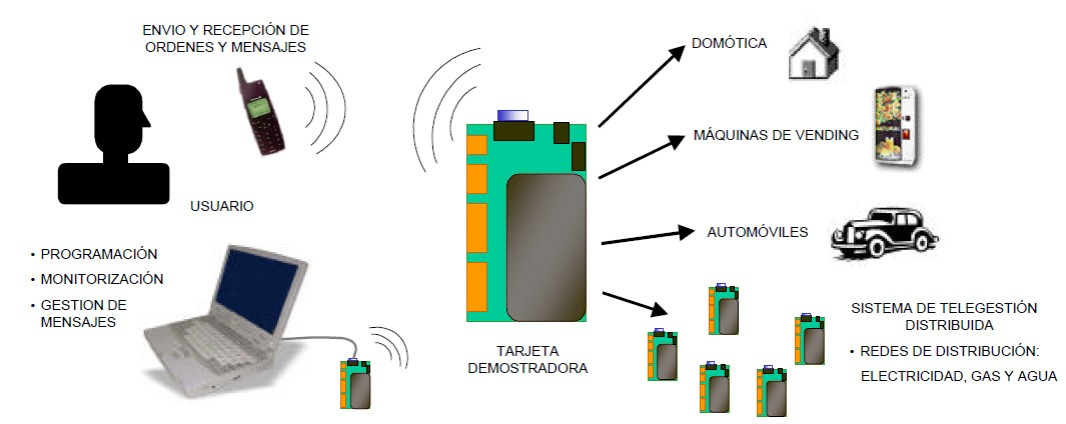
\includegraphics[width=1\textwidth]{introduccion/fig3.jpg}
\caption{Esquema del funcionamiento del sistema de telecontrol \cite{UPS-05}. }
\label{Ftres}
\end{figure}
%

Existe una gran cantidad de proyectos que se pueden implementar en diferentes equipos (\cite{UPS-05,UPS-06}). En el caso de los vehículos, Luis Miguel Ruiz (\cite{UPS-06}) en septiembre del 2015 presentó su tema de fin de grado el cual describe la instalación de sistemas de seguridad pasiva en un vehículo clásico perteneciente a la gama baja. Él explica que estos sistemas están conformados de tecnología accesible en estos tiempos, Luis la implementa en un vehículo MINI MORRIS 850 de 1972. Dichos sistemas son: i) alarma antirrobo, ii) ayuda al estacionarse, iii) monitorización de las revoluciones del motor y iv) encendido automático de luces. Este tema se ha llevado acabo principalmente con relevadores, sensores de distancia y la tarjeta programable Arduino, desarrollando un diagrama de flujo para plasmar las actividades generales como se muestra en la Figura \ref{Ftresdos}, sin embargo, a pesar de que es una idea muy interesante puede carecer de detalles de análisis para controlar los sistemas de una manera más eficiente, sin mencionar la cantidad de proyectos realizados similares con la tarjeta Arduino.\\

%
\begin{figure}[H]
%\vspace{0.2cm}
\centering
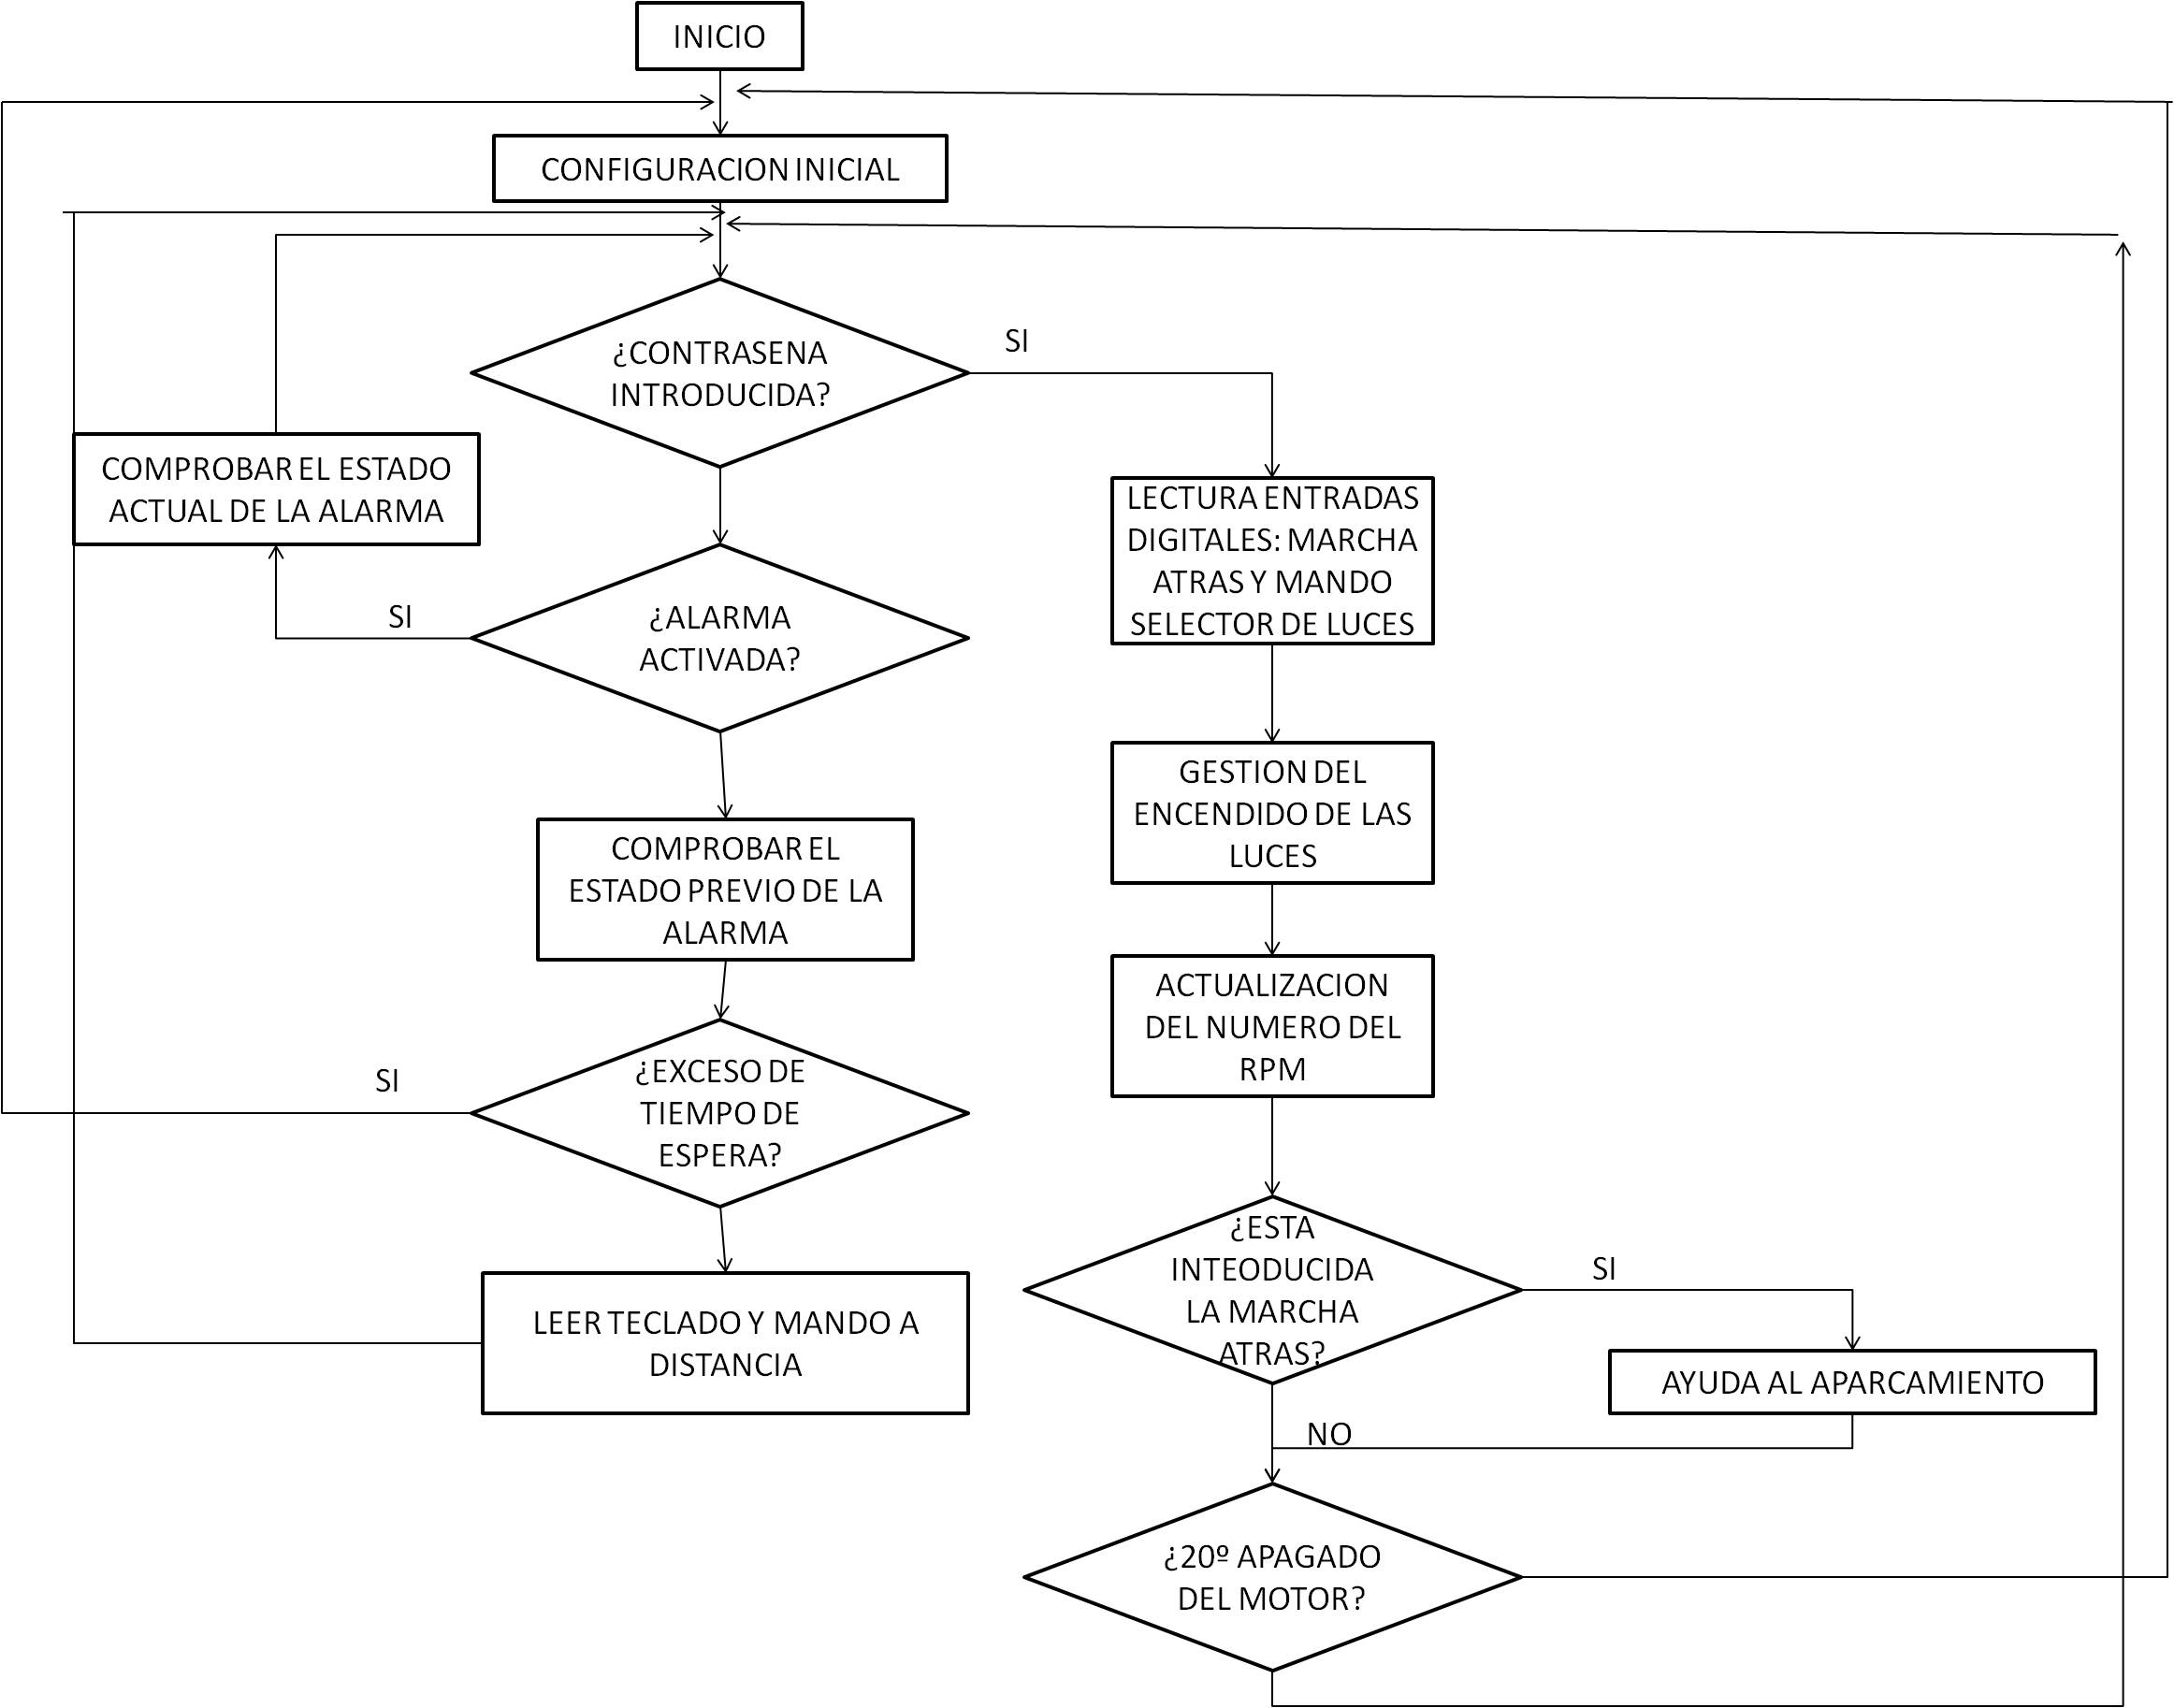
\includegraphics[width=0.8\textwidth]{introduccion/fig5.jpg}
\caption{Vista general del diagrama de flujo del programa. }
\label{Ftresdos}
\end{figure}
%

Por otra parte, existen aplicaciones móviles enfocadas en vehículos de gama media y alta (\cite{UPS-07,UPS-08}), los vehículos definidos en estas gamas contienen el sistema diagnóstico a bordo II (OBD del inglés \textit{On Board Diagnostic}). El sistema \textit{OBD} permite la comunicación entre los sensores del sistema de tracción. Miriam Loachamín en octubre del 2015 (\cite{UPS-07}) desarrollo su trabajo enfocado al monitoreo de parámetros mediante el dispositivo Arduino y la librería OBD.h, donde esta permite la lectura de códigos del sistema \textit{OBD II}. El dispositivo Arduino envía y recibe la señal con la tecnología de comunicación de los celulares GSM y lo representa por medio de un diagrama de bloques del sistema, el cual se muestra en la Figura \ref{Fcuatro}. Por otro lado, el dispositivo ELM 327 se inserta en el conector de enlace de datos para enviar las señales que obtiene de los sensores del vehículo. El ELM 327 únicamente permite únicamente el monitoreo de ciertos sensores del sistema de tracción del vehículo, no permite la comunicación con actuadores para su manipulación.\\

%
\begin{figure}[H]
%\vspace{0.2cm}
\centering
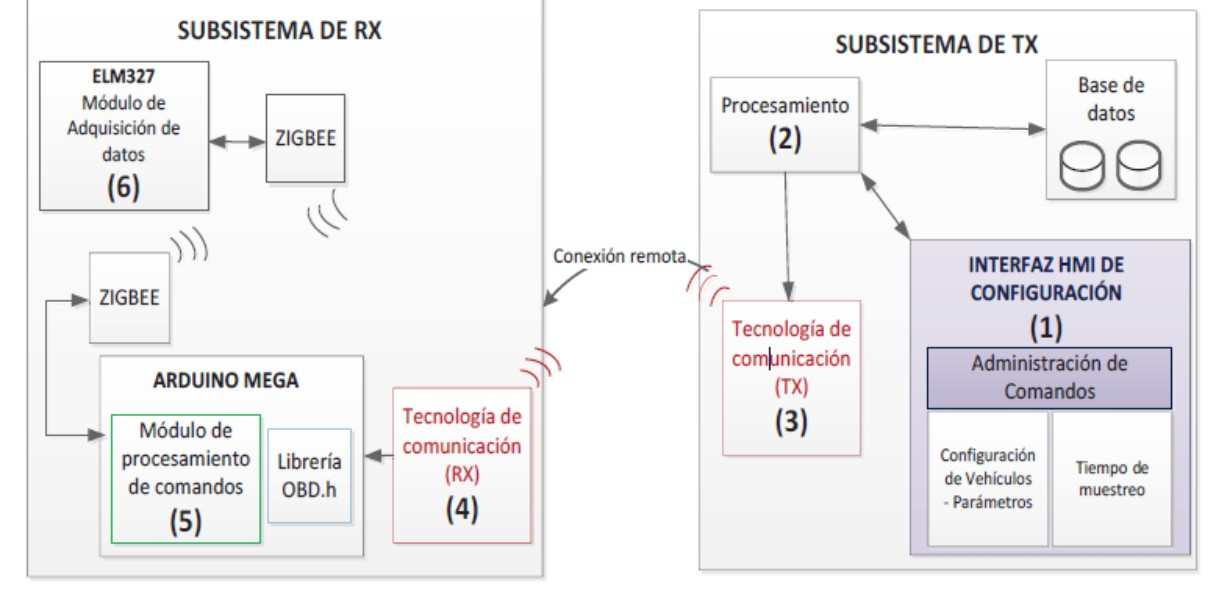
\includegraphics[width=0.8\textwidth]{introduccion/fig6.jpg}
\caption{Diagrama de bloques del sistema de administración remota propuesto \cite{UPS-07}. }
\label{Fcuatro}
\end{figure}
%


En septiembre del 2015 Virgilio García trabajó con un vehículo (\cite{UPS-08}), utilizó la tarjeta electrónica ELM 327 junto con una tarjeta Raspberry Pi que implemento al vehículo. Esta adaptación permitió incorporar de manera independiente al vehículo, los sensores de temperatura y monóxido de carbono, con un sistema de notificación en caso de información inusual. Virgilio se basa principalmente en el desarrollo de una aplicación móvil para sistema operativo Android en donde puede medir la temperatura interior con un historial de la temperatura por fecha, tal como se muestra en la Figura \ref{Fcinco}, donde utiliza la tecnología Bluetooth como medio de comunicación. Este trabajo al igual que el tema de Miriam Loachamín utilizan la librería OBD.h que contiene la información de los códigos del sistema de tracción, aunque no permite la modificación de ningún parámetro del sensor o actuador, simplemente es el monitoreo de ciertos sensores dependiendo el vehículo.\\

%
\begin{figure}[H]
%\vspace{0.2cm}
\centering
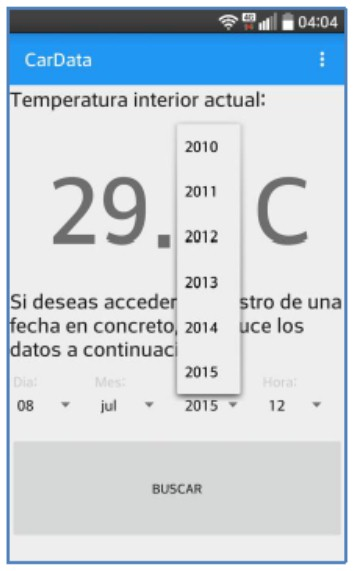
\includegraphics[width=0.3\textwidth]{introduccion/fig7.jpg}
\caption{Interaz que muestra el historial de la temperatura del vehículo \cite{UPS-08}. }
\label{Fcinco}
\end{figure}
%

Jesús Castillo y colaboradores trabajaron en el 2015 (\cite{UPS-10}), con el tema relacionado al sistema de seguridad activa que comprende de los sistemas antibloqueo de frenos, control de tracción y de control de estabilidad. Proponen detectar las condiciones de la carretera por donde pasa el vehículo utilizando sensores estándar como los vehículos, buscando estimaciones en tiempo real sobre la fuerza de contacto entre la rueda, la carretera y la velocidad. Obtuvieron un algoritmo de estimación de parámetros y mediante leyes físicas y cálculos matemáticos realizaron un esquema de cálculo, tal cual se muestra en la Figura \ref{Fcincodos} para obtener el deslizamiento y el coeficiente de fricción y a partir de esos datos el estado de la carretera y el deslizamiento óptimo de la superficie en la que el vehículo está circulando. Además, estos parámetros son fundamentales para los sistemas de seguridad activa o de la conducción automática del controlador para una reacción más rápida y con más facilidad a situaciones inesperadas y peligrosas.\\

%
\begin{figure}[H]
%\vspace{0.2cm}
\centering
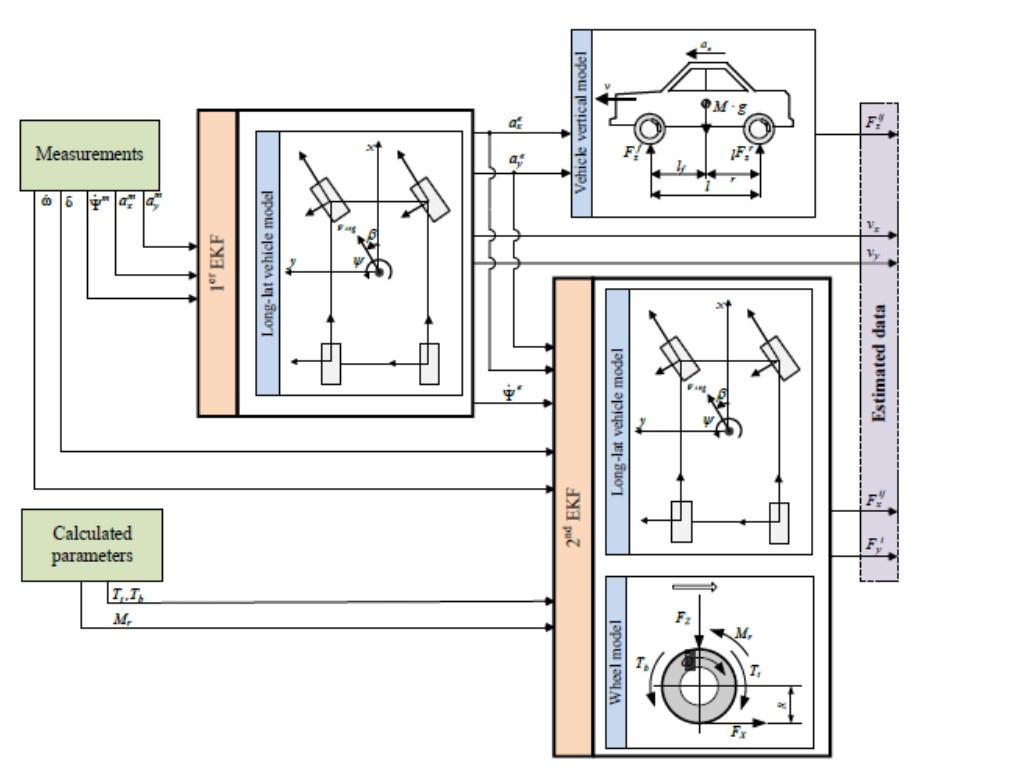
\includegraphics[width=0.7\textwidth]{introduccion/fig8.jpg}
\caption{Esquema del algoritmo estimado \cite{UPS-10}. }
\label{Fcincodos}
\end{figure}
%


En el 2012 se presentó un artículo a cargo de Jorge Capra y colaboradores (\cite{UPS-13}), sobre la detección de vehículos robados en Argentina, por medio del reconocimiento automático de las placas usando un reconocedor óptico tal cual se muestra en la Figura \ref{Fseis}. Sin embargo, gran parte del trabajo se realizó en un ambiente controlado y existen dificultades para detectar caracteres cuando hay poco contraste o la iluminación no es homogénea o con demasiada perspectiva. Este trabajo puede tener varias funcionalidades además del control vehicular como por ejemplo, en operativos de inspección policial, identificación en puestos de peajes y control de estacionamiento, entre otros.\\

%
\begin{figure}[H]
%\vspace{0.2cm}
\centering
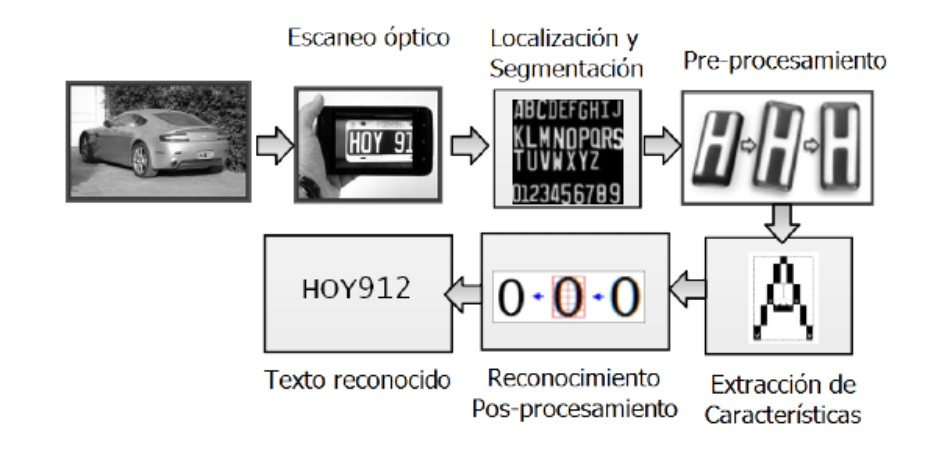
\includegraphics[width=0.7\textwidth]{introduccion/fig9.jpg}
\caption{Esquema del algoritmo estimado \cite{UPS-13}. }
\label{Fseis}
\end{figure}
%

El bloqueo y desbloqueo electrónico por huella dactilar es un proyecto de Luis Eduardo Cando (\cite{UPS-09} ), en donde se pretende tener un mayor nivel de seguridad al instante de encender el automóvil, mediante un módulo biométrico y una pantalla para visualizar la interfaz entre el vehículo y el módulo, buscando el encendido del vehículo soló por personas dadas de alta en el sistema de control. Las pruebas que se realizaron en este trabajo describen el buen funcionamiento de la huella o conocer el código pin del módulo biométrico, mostrando el diagrama general, además del costo equivalente a  837.70 USD para la implementación del proyecto. Sin embargo, para este proyecto es indispensable los relevadores automotrices, dejando la oportunidad a un experto en mecánica o electrónica poder desconectar con facilidad la seguridad.\\


Edwin Ismael en diciembre del 2015 (\cite{UPS-11}), trabajó en un proyecto para el control del sistema de iluminación, accionamiento de ventanillas, limpiaparabrisas, calefacción por medio de comandos de voz y una tarjeta electrónica con base en Arduino. En las conclusiones muestran la necesidad de un acumulador en buen estado y habla sobre las limitaciones actuales del comando por voz, debido a que existen muchos factores que alteran la tonalidad de la voz provocando dificultades para ejecutar los comandos. \\


En el 2013 Oswaldo Quito y Benito Sarmiento (\cite{UPS-12}), desarrollaron un sistema para obtener su grado de ingeniería donde controlan algunas actividades del vehículo Luv Clásica de la marca Chevrolet mediante SMS, utiliza la tecnología GPS para localizar la camioneta cuando se requiera. De igual forma se puede bloquear por medio del GPS en cualquier lugar donde se encuentre. Oswaldo y Benito nos muestran su esquema general en la Figura \ref{Fnueve}, también corta el combustible directamente de la camioneta, además de un panel para configurar el sistema y por medio de un relevador se puede bloquear el encendido electrónico.\\

%
\begin{figure}[H]
%\vspace{0.2cm}
\centering
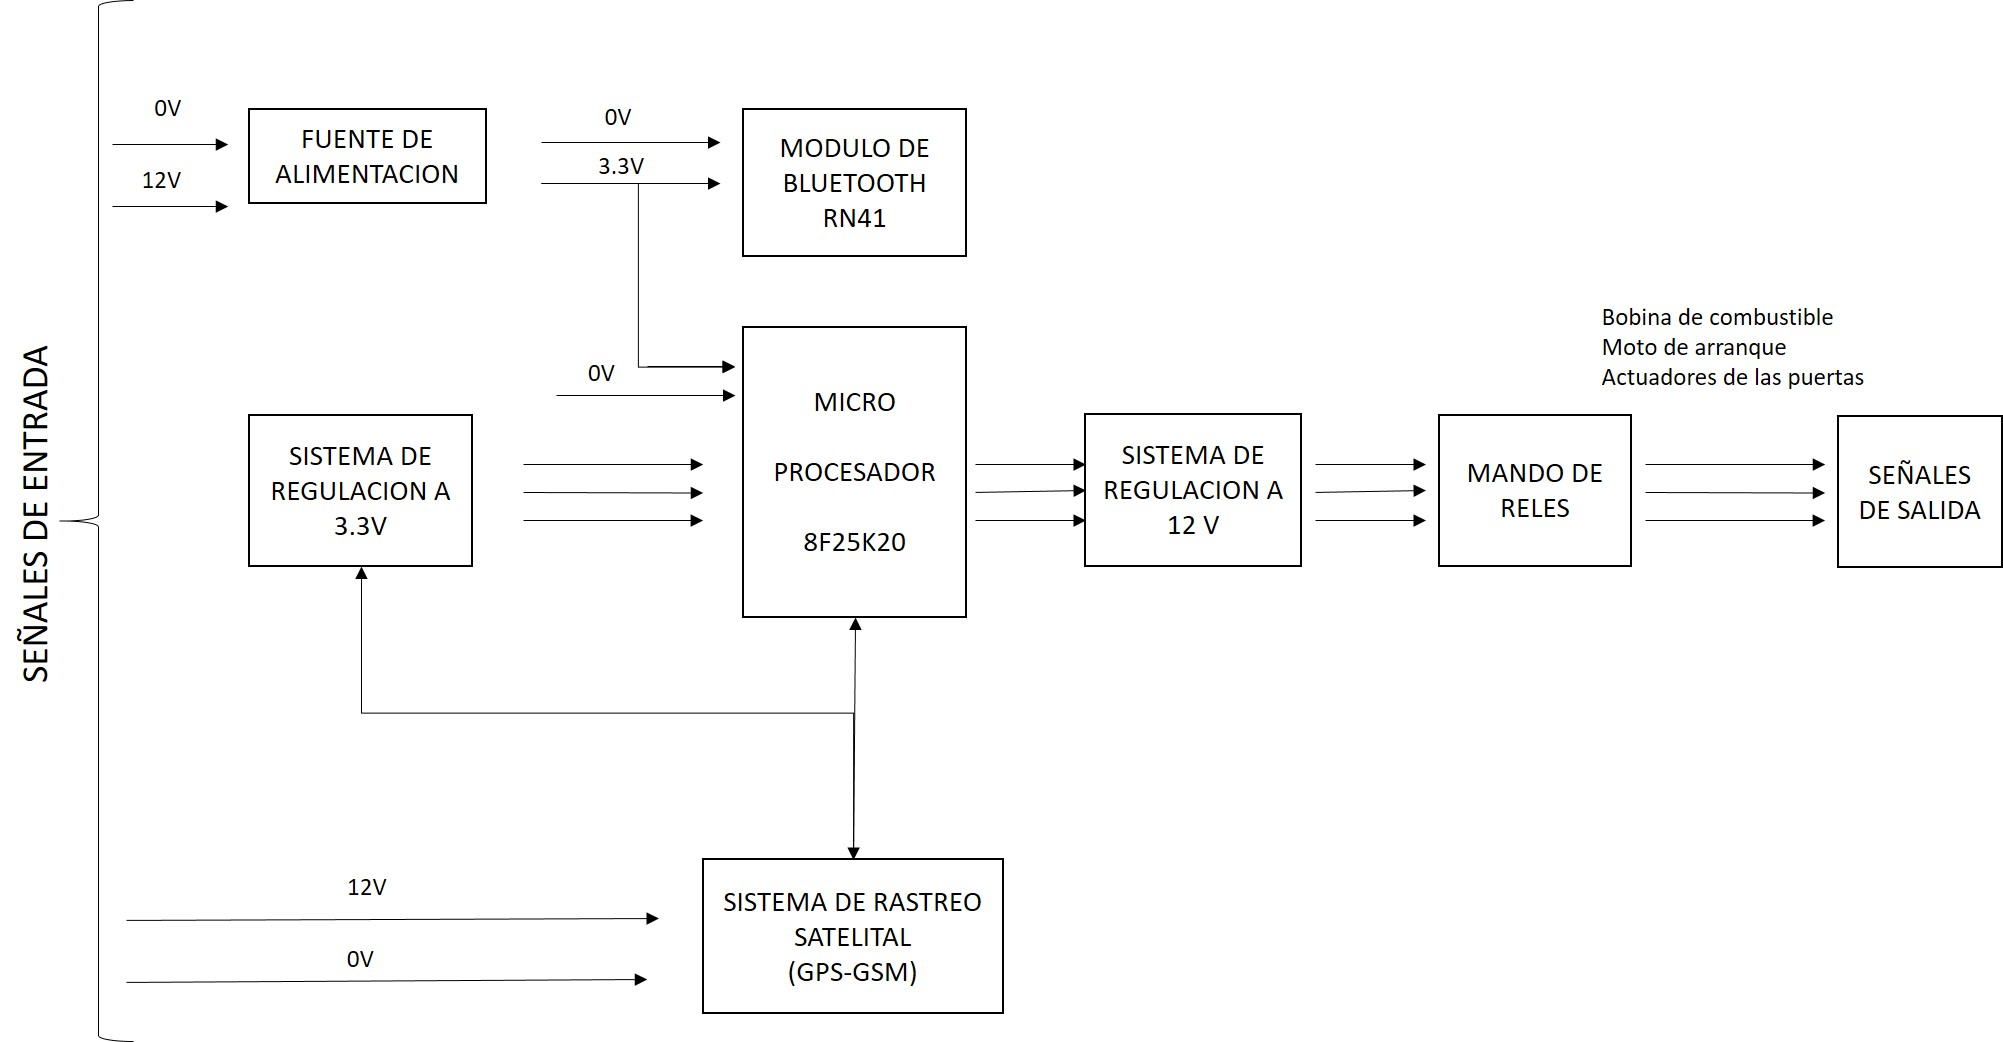
\includegraphics[width=0.6\textwidth]{introduccion/fig12.jpg}
\caption{Esquema del circuito electrónico \cite{UPS-12}. }
\label{Fnueve}
\end{figure}
%

Roberto Carlos Paredes (\cite{UPS-14}), trabajo en el 2014 con un proyecto de seguridad, que permite detectar mediante sensores de presión cuando una persona está ocupando el asiento del piloto o copiloto y con un sensor de proximidad magnético se puede identificar si la persona tiene puesto el cinturón de seguridad cuando el vehículo ya este encendido, utilizando un sistema de reproducción MP3 para emitir un aviso. Roberto nos muestra una imagen de la implementación en la Figura \ref{Fdiez}\\

%
\begin{figure}[H]
%\vspace{0.2cm}
\centering
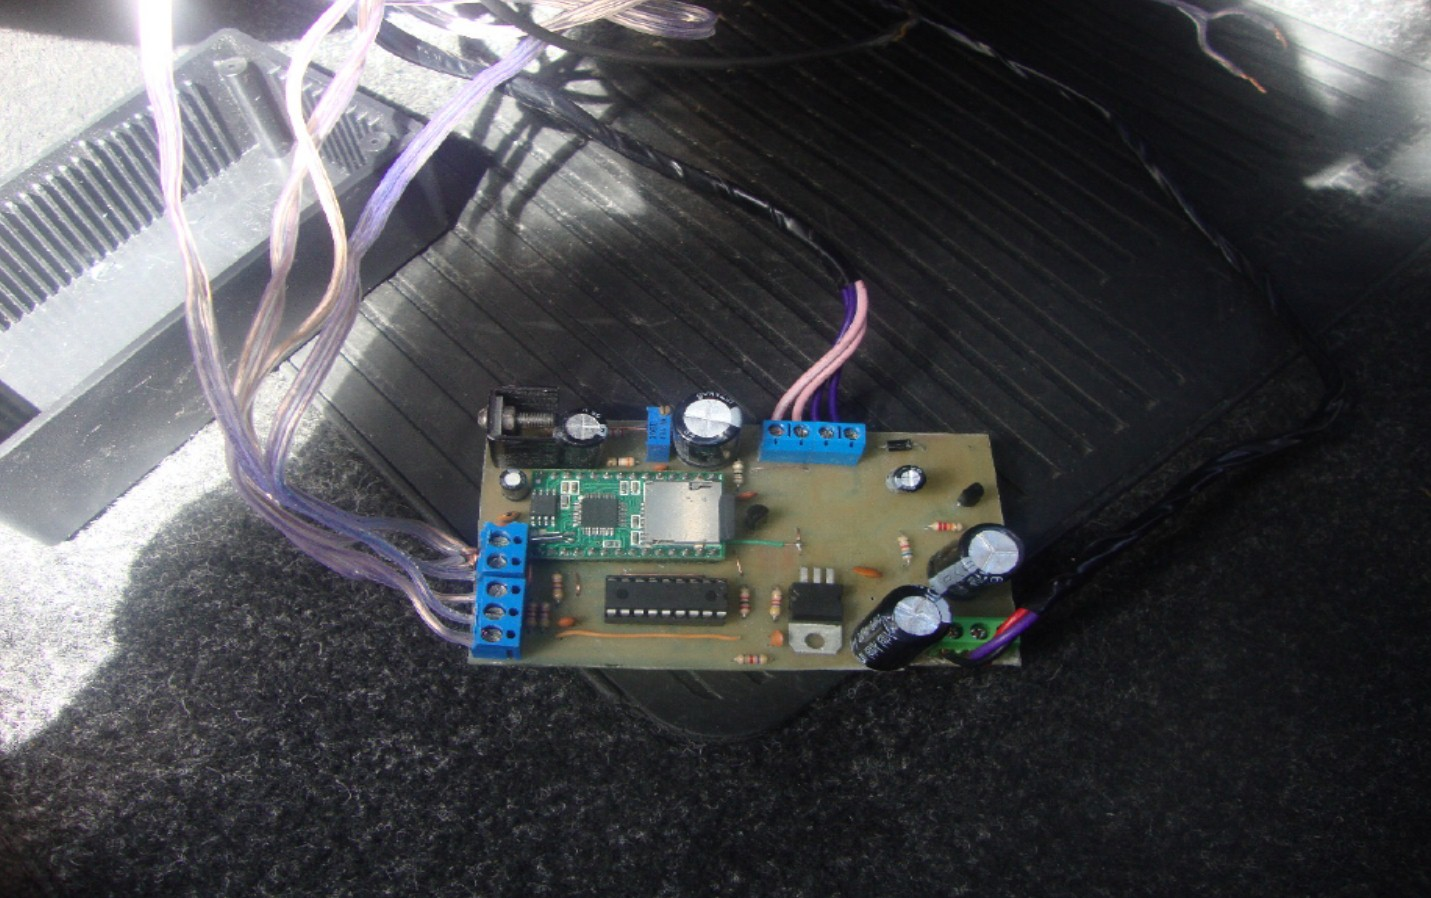
\includegraphics[width=0.6\textwidth]{introduccion/fig13.jpg}
\caption{Placa electrónica Conectada al vehículo \cite{UPS-14}. }
\label{Fdiez}
\end{figure}
%

Otro de los trabajos que se realizó fueron algunas actividades con el sistema \textit{OBD} II y el \textit{CAN-BUS} de datos (\cite{GB1}), desarrollando la siguiente hipotesis. La solución que se propone es el desarrollo de una aplicación móvil mediante plataforma Android para poder modificar algunos parámetros y sensores del Sistema de Confort de un Vehículo de Gama media, utilizando de vehículo de pruebas un Stratus XLS 2006. \\

Las actividades que se desarrollaron fueron enfocadas a realizar pruebas en sistemas existentes en el mercado, estas se enlistan acotinuación:

\begin{itemize}
\item Funcionamiento del Can Bus y el conector DCL,
\item Funcionamiento del dispositivo EML327,
\item Funcionamiento de aplicaciones móviles,
\item Codificación y descodificación de la señal,
\item Pruebas y Resultados.
\end{itemize}

\paragraph{Funcionamiento del Can Bus y el conector DCL}
El desarrollo de esta actividad se llevó a cabo mediante la investigación de la metodología sobre el Sistema eléctrico del vehículo (\cite{GB1}), el can bus es el encargado de transmitir los códigos de falla del vehículo y el conector OBD, también conocido como conector de enlace de datos es el encargado pasar por medio de algún escáner los códigos al usuario, está ubicado normalmente en la parte inferior del volante.\\

Durante esta actividad también se realizaron pruebas con el osciloscopio, detectando los pines encargados de transmitir las señales por medio del CAN Bus, también denominados CAN \textit{High} y CAN \textit{Low}, los pines correspondientes son el número 2 y el 10, tal y como se muestra en la Figura \ref{Medos} debido a que cada marca maneja un protocolo ya establecido.

%
\begin{figure}[H]
%\vspace{0.2cm}
\centering
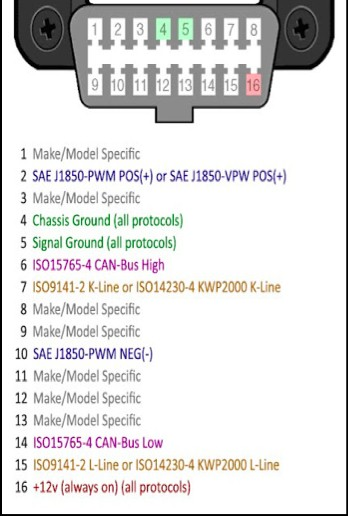
\includegraphics[width=0.3\textwidth]{metodologia/protocolos_obd.jpg}
\caption{Protocolos de comunicación con la configuración de los pines del conector DCL.}
\label{Medos}
\end{figure}
%

\paragraph{Funcionamiento del dispositivo EML327}

En la siguiente actividad se probaron algunas aplicaciones móviles existentes en el mercado para poder verificar por cuenta propia que el sistema Can Bus es capaz de enviar información relevante para el usuario a la hora de viajar en el vehículo (\cite{GB2}).\\

Por lo cual se realizaron pruebas con el escáner EML327, sin embargo este escáner funciona únicamente  para el sistema de tracción, esto permitió realizar las primeras pruebas en el vehículo sobre el escaneo de información a una aplicación móvil mediante tecnología Bluetooth. \\

Primeramente se conectó el EML327 al conector de enlace de datos tal cual se muestra en la Figura \ref{Metres}\\

%
\begin{figure}[H]
%\vspace{0.2cm}
\centering
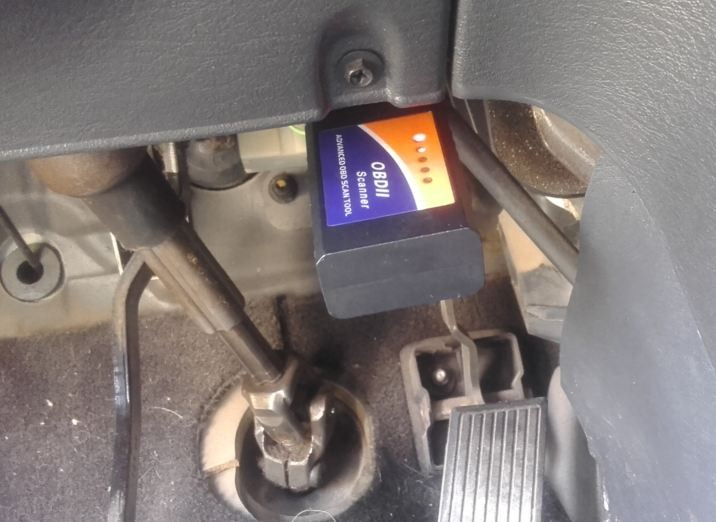
\includegraphics[width=0.5\textwidth]{metodologia/elm327.jpg}
\caption{dispositivo EML 327 conectado al vehículo.}
\label{Metres}
\end{figure}


\paragraph{Funcionamiento de aplicaciones móviles}

Después se buscó en la tienda de Google Play aplicaciones compatibles con el escáner EML327, se obtuvieron dos aplicaciones``Scanner OBD" y ``Piston”, se descargaron y se procedió a visualizar el funcionamiento de ambas. La aplicación Escáner OBD muestra información sobre el protocolo de comunicación la cual se muestran en las Figuras \ref{Mecuatro}. 

\begin{figure}[H]
\centering
\subfigure[]{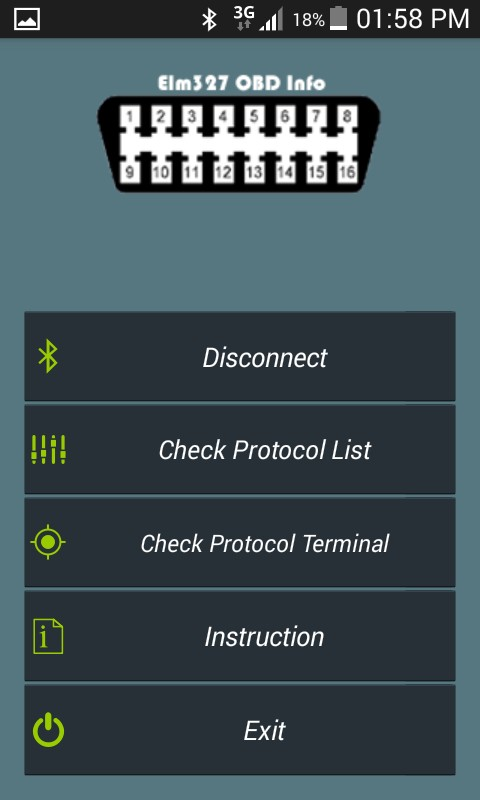
\includegraphics[width=60mm]{metodologia/eml327.jpg}}\hspace{10mm}
\subfigure[]{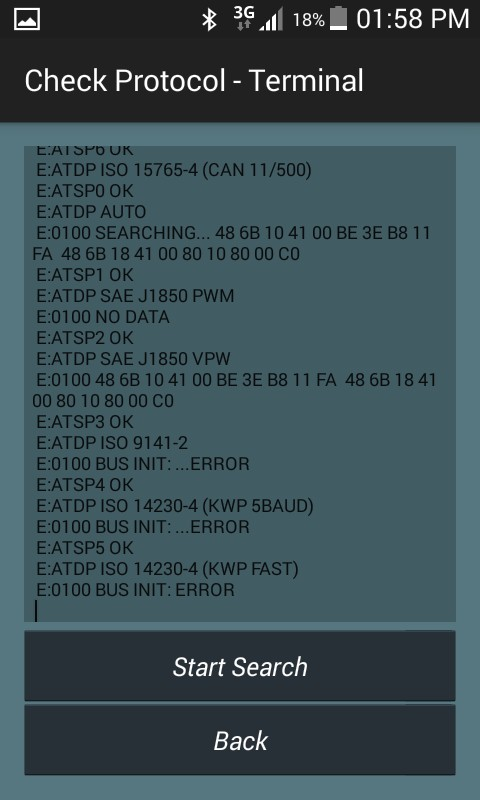
\includegraphics[width=60mm]{metodologia/eml327_.jpg}}
\caption{Pantallazos de la aplicación Scanner OBD.} \label{Mecuatro}
\end{figure}


La aplicación “Piston” muestra información sobre el sistema de tracción como el voltaje de la batería, la temperatura del agua, las revoluciones por minuto y la velocidad, tal cual se muestra en la Figura \ref{Mecinco}.

\begin{figure}[H]
\centering
{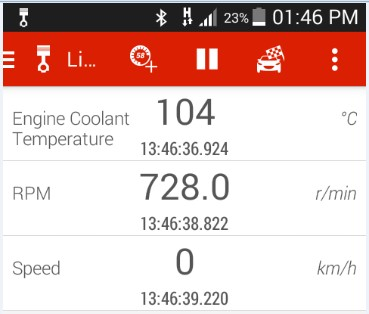
\includegraphics[width=0.6\textwidth]{metodologia/piston.jpg}}
\caption{Pantallazo de la aplicación Piston.} \label{Mecinco}
\end{figure}



\paragraph{Codificación y descodificación de la señal}

Para esta actividad, se vio en la necesidad de conocer completamente el sistema de confort, principalmente en la parte del sistema eléctrico. \\

Por protocolos de seguridad las armadoras no permiten el acceso al mismo, sin embargo algunas asociaciones de mecánicos en el país tienen acceso a ellos mediante software que los auxilia a reparar los vehículo, como es el caso del software OnDemand5 (\cite{GB3}).\\


\subsection{OBJETIVOS}
\subsubsection{Objetivo General}
Incrementar la comodidad y la seguridad de vehículos de gama baja mediante la implementación de actuadores manipulados por una aplicación móvil para el monitoreo de la emisión de algunos gases y aumentar la comodidad y seguridad del tripulante.


\subsubsection{Metas específicas}
  \begin{itemize}
           \item Diseñar una estructura de comunicación entre los actuadores y la aplicación móvil
\item Instrumentar los actuadores seleccionados
\item Diseñar el circuito electrónico
\item Desarrollar la aplicación móvil
  \end{itemize}



\subsection{SOLUCIÓN PROPUESTA}
Desarrollar una metodología que permita aumentar la comodidad y seguridad para el tripulante por medio de la incorporación de tecnología en vehículos de gama baja y modelos anteriores.\\

Mediante la tecnología de bluetooth se comunica una aplicación móvil a una tarjeta electrónica dentro del vehículo que permita manipular los actuadores del vehículo pertenecientes al sistema de confort y tracción del vehículo.\\
